% AI Clinic Research Report — compile with pdflatex (run twice)
\documentclass[11pt,a4paper]{article}

\usepackage[margin=2.5cm]{geometry}
\usepackage[utf8]{inputenc}
\usepackage[T1]{fontenc}
\usepackage{lmodern}
\usepackage{graphicx}
\usepackage{amsmath,amssymb}
\usepackage{booktabs}
\usepackage{xcolor}
\usepackage{fancyhdr}
\usepackage{caption}
\usepackage[colorlinks=true,linkcolor=blue!50!black,citecolor=blue!50!black,urlcolor=blue!60!black]{hyperref}

\definecolor{aivblue}{HTML}{0B3D5C}
\definecolor{aivteal}{HTML}{00A98F}

\captionsetup{font=small,labelfont=bf}

% Allow figure-dense pages so floats stay near their text
\renewcommand{\topfraction}{0.9}
\renewcommand{\bottomfraction}{0.8}
\renewcommand{\textfraction}{0.07}
\renewcommand{\floatpagefraction}{0.8}

\pagestyle{fancy}
\fancyhf{}
\fancyhead[L]{\small\color{aivblue} PGE5 --- AI Clinic Research Report}
\fancyhead[R]{\small\color{aivblue} aivancity}
\fancyfoot[C]{\small\thepage}
\renewcommand{\headrulewidth}{0.4pt}

\newcommand{\bd}{\bar{d}}

\begin{document}

% ============================ TITLE PAGE ============================
\begin{titlepage}
    \centering
    
\includegraphics[width=0.35\textwidth]{../assets/aivancity_logo.png}\\[1.2cm]

    {\color{aivblue}\rule{\textwidth}{1.2pt}}\\[0.9cm]

    {\LARGE\bfseries\color{aivblue}
    CNN-Adaptive Sliding Mode Control and Reinforcement Learning
    for Autonomous Differential-Drive Robots\\[0.35cm]}
    {\Large\color{aivblue} Under Environmental Uncertainty --- A Digital Twin Approach\\[0.6cm]}

    {\color{aivblue}\rule{\textwidth}{1.2pt}}\\[1.4cm]

    {\large\itshape AI Clinic Research Project Report}\\[0.3cm]
    {\large PGE5 --- Programme Grande \'Ecole}\\[1.6cm]

    \begin{tabular}{r l}
        \textbf{Participating Students:} & Likhita Yerra \\
                                         & Mohamed Oussama Bouriga \\
                                         & Ahmed Ben Aissa \\
                                         & Abdellahi El Moustapha \\
                                         & Thibault Goutorbe \\[0.5cm]
        \textbf{Supervisor:}             & Prof.\ Vishvjit Thakar \\[0.5cm]
        \textbf{Date of Submission:}     & 30 August 2026 \\
    \end{tabular}\\[1.8cm]

    {\small aivancity --- School of Technology and Management for AI, Paris, France}

    \vfill
\end{titlepage}

% ============================ ABSTRACT ============================
\begin{abstract}
\noindent
Fixed-gain Sliding Mode Control (SMC) cannot simultaneously optimise chattering
suppression and disturbance rejection across diverse operating conditions. We propose
a CNN-adaptive SMC framework in which a lightweight convolutional network classifies
the pre-mission environment from a $64{\times}64$ occupancy map and selects a hand-tuned
SMC parameter preset at run time. Five uncertainty scenarios are evaluated on a simulated
differential-drive robot against classical SMC and three adaptive baselines: fuzzy gain
scheduling, oracle map classification, and reinforcement-learning preset selection.
CNN-adaptive SMC reduces angular-velocity chattering by 35.7\% under sensor noise and
improves final tracking-error recovery by up to 32.7\% under wheel slip and 14.4\% under
impulsive disturbance, approaching oracle performance (17.9\,mm vs.\ 15.6\,mm). On
realistic occupancy maps, EnvironmentCNN reaches 95.1\% classification accuracy. The
complete pipeline is integrated into a real-time 3D digital twin for live demonstration,
controller comparison, and replay.
\end{abstract}

\vspace{0.3cm}
\noindent\textbf{Keywords:} sliding mode control, adaptive control, convolutional neural
network, reinforcement learning, gain scheduling, mobile robot, chattering reduction,
digital twin.

\vspace{0.5cm}
\tableofcontents
\newpage

% ============================ INTRODUCTION ============================
\section{Introduction}

\subsection{Problem Statement}

Autonomous mobile robots navigating in unstructured environments must maintain accurate
trajectory tracking despite sensor noise, mechanical disturbances, and surface-induced
wheel slip. Sliding Mode Control (SMC) is widely adopted in this domain because of its
intrinsic robustness to matched disturbances and parameter variations
\cite{utkin1992,edwards1998}. However, classical SMC uses a single fixed set of gains
that cannot simultaneously optimise chattering suppression, tracking accuracy, and
disturbance rejection across all operating regimes: noisy sensors call for smoother,
lower-bandwidth actuation, whereas impulsive pushes and wheel slip call for aggressive
corrective gains.

This project addresses the research question: \emph{can a learning-based perception and
control pipeline improve the adaptability of sliding mode control for a differential-drive
mobile robot under heterogeneous uncertainty conditions?} Our contributions are:

\begin{itemize}
    \item A complete, reproducible CNN-adaptive SMC pipeline from synthetic map generation
          and CNN training through simulation and quantitative evaluation.
    \item An \emph{EnvironmentCNN} that classifies five scenario types from occupancy maps,
          with 100\% test accuracy on engineered simple maps and 95.1\% on realistic maps,
          supported by baseline classifier comparisons.
    \item A multi-controller benchmark against fuzzy-SMC, oracle selection, and RL-adaptive
          SMC under identical simulation conditions, showing CNN supervision near the
          oracle ceiling.
    \item Quantitative analysis of the tracking--smoothness trade-off: scenario-aware
          presets reduce chattering by up to 35.7\% while preserving interpretable,
          certifiable gain schedules.
    \item A real-time 3D \emph{digital twin} (React + Three.js frontend, FastAPI WebSocket
          backend) providing live visualisation, controller tours, side-by-side comparison,
          replay, and metric export for demonstration and defense.
\end{itemize}

\begin{figure}[ht]
    \centering
    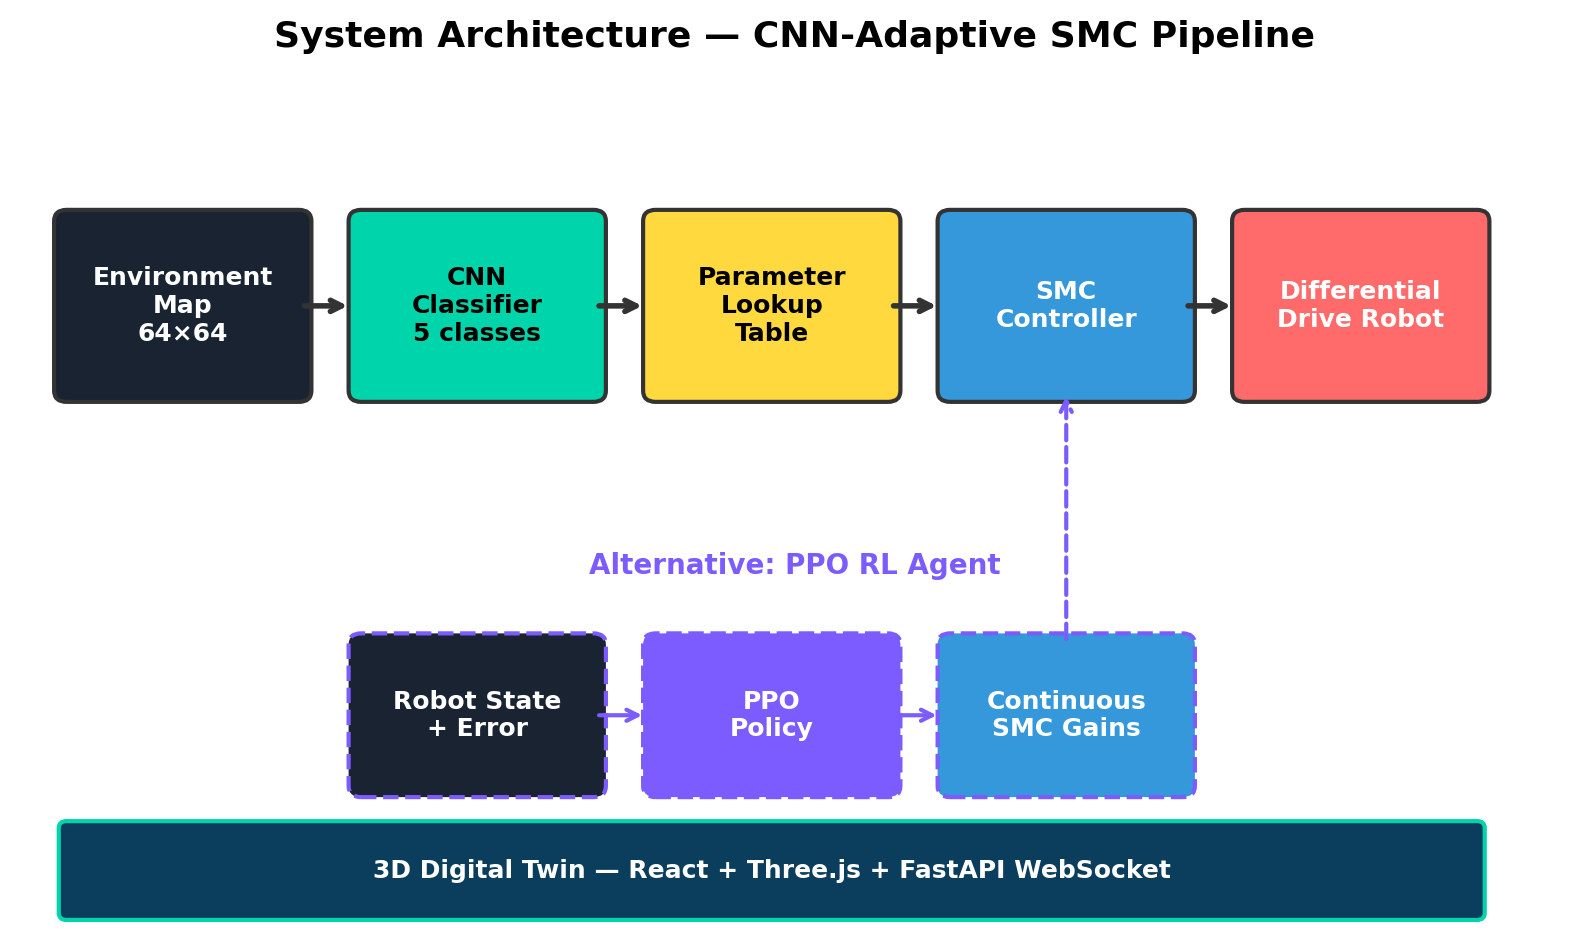
\includegraphics[width=0.95\textwidth]{../assets/figures/fig01_architecture.png}
    \caption{System architecture: the CNN-adaptive SMC pipeline (top) and the PPO
    reinforcement-learning alternative (bottom), both integrated into the 3D digital twin.}
    \label{fig:architecture}
\end{figure}

\subsection{Literature Review}

\paragraph{Sliding Mode Control for Mobile Robots.}
SMC provides finite-time convergence and robustness to matched uncertainties
\cite{utkin1992}. Anti-chattering techniques, including boundary layers, saturation
switching, and higher-order SMC, are well established \cite{shtessel2014,slotine1991}.
Adaptive SMC with Lyapunov-based gain tuning can converge slowly or require tight
disturbance bounds \cite{edwards1998}. Differential-drive platforms in particular benefit
from SMC due to their nonholonomic constraints and sensitivity to lateral disturbances
\cite{edwards1998,slotine1991}.

\paragraph{Learning-Based Gain Adaptation.}
Fuzzy-SMC hybrids \cite{lin2006} and radial-basis-function networks \cite{ge2004} tune
switching gains automatically, removing the need for manual tuning. Reinforcement learning
combined with SMC has been explored for aerial \cite{nguyen2018} and manipulation
platforms, though sample efficiency remains a practical concern for physical deployment.
A key limitation of pure learning-based approaches is their opacity: the resulting gain
schedules are difficult to interpret or certify, which motivates our use of hand-tuned
presets selected by a learned classifier.

\paragraph{CNN-Based Supervisory Control.}
Supervisory switching architectures that select among pre-designed controllers based on a
mode estimate are established in hybrid and switched systems theory \cite{liberzon2003}.
CNN-based perception has been widely adopted for environment understanding in autonomous
navigation \cite{lecun2015,levine2016}, yet its direct use as a gain-scheduling oracle for
SMC has received comparatively little attention. Our approach bridges this gap, using a
lightweight CNN to classify a pre-mission occupancy map and drive SMC parameter selection,
combining the interpretability of hand-tuned presets with the representational power of
deep features.

\paragraph{Digital Twins.}
Digital twin technology provides a virtual replica of a physical system for monitoring,
simulation, and decision support. For robotics research, a web-based 3D twin enables live
demonstration of control algorithms, side-by-side controller comparison, and stakeholder
communication --- capabilities we exploit for the AI Clinic defense.

% ============================ METHODOLOGY ============================
\section{Methodology}

\subsection{Differential-Drive Robot Model}

The robot is modelled as a unicycle differential-drive with state
$q = [x, y, \theta, v, \omega]^{\top}$, where $(x, y)$ is the Cartesian position,
$\theta$ the heading, $v$ the linear velocity, and $\omega$ the angular velocity.
The continuous-time kinematics are
\begin{equation}
    \dot{x} = v\cos\theta, \qquad \dot{y} = v\sin\theta, \qquad \dot{\theta} = \omega .
    \label{eq:kinematics}
\end{equation}
Discrete integration with step $\Delta t = 0.01$\,s uses the Euler method. Physical
parameters: wheel base $L = 0.3$\,m, wheel radius $r = 0.05$\,m. The differential drive
imposes the nonholonomic constraint $\dot{y}\cos\theta - \dot{x}\sin\theta = 0$: the
robot cannot move laterally, making lateral disturbances particularly challenging to
reject and motivating the sliding-surface design below.

\subsection{Classical Sliding Mode Controller}

Tracking errors are $e_x = x_r - x$, $e_y = y_r - y$, $e_\theta = \theta_r - \theta$
(angles normalised to $(-\pi, \pi]$). Sliding surfaces are
\begin{equation}
    s_i = \dot{e}_i + \lambda_i e_i, \qquad i \in \{x, y, \theta\},
    \label{eq:surfaces}
\end{equation}
with $\lambda_i > 0$ and finite-difference derivative approximations.
The linear velocity command tracks the projected forward error:
\begin{equation}
    v_c = v_r + k_v d_f, \qquad d_f = \cos\theta\, e_x + \sin\theta\, e_y ,
    \label{eq:vc}
\end{equation}
where $v_r$ is the reference speed. The raw angular-velocity command combines a bearing
correction and two sliding-surface switching terms:
\begin{equation}
    \omega_{\text{raw}} = k_\omega \left[ \psi
        + \tanh\!\left(\frac{s_y}{\varphi}\right)
        + 0.2\tanh\!\left(\frac{s_\theta}{\varphi}\right) \right],
    \label{eq:omega}
\end{equation}
where $\psi = \operatorname{atan2}(e_y, e_x) - \theta$ is the bearing angle and $\varphi$
the boundary-layer width. The hyperbolic-tangent switching function replaces the
discontinuous sign function to suppress chattering \cite{shtessel2014}. An exponential
smoother with coefficient $\alpha_\omega$ further attenuates high-frequency oscillation:
\begin{equation}
    \omega_c = \alpha_\omega\, \omega_{c,k-1} + (1 - \alpha_\omega)\, \omega_{\text{raw}} .
    \label{eq:smoother}
\end{equation}
Both $v_c$ and $\omega_c$ are clipped to hardware limits; dead zones
($|d_f| < 0.01$\,m, $|e_\theta| < 0.01$\,rad) suppress spurious switching near the
reference.

\subsection{CNN Environment Classifier}

\paragraph{Dataset.}
Synthetic $64 \times 64$ grayscale maps are generated for five classes: \emph{Normal}
(clean path line), \emph{Noise} (noisy pixel overlay), \emph{Disturbance} (off-path impact
marker), \emph{Slip} (shaded low-friction zone), and \emph{Combined} (all effects), as
shown in Fig.~\ref{fig:cnnsamples}. The dataset contains 1{,}500 samples (300 per class)
split 70\%/15\%/15\% for training, validation, and testing.

\begin{figure}[ht]
    \centering
    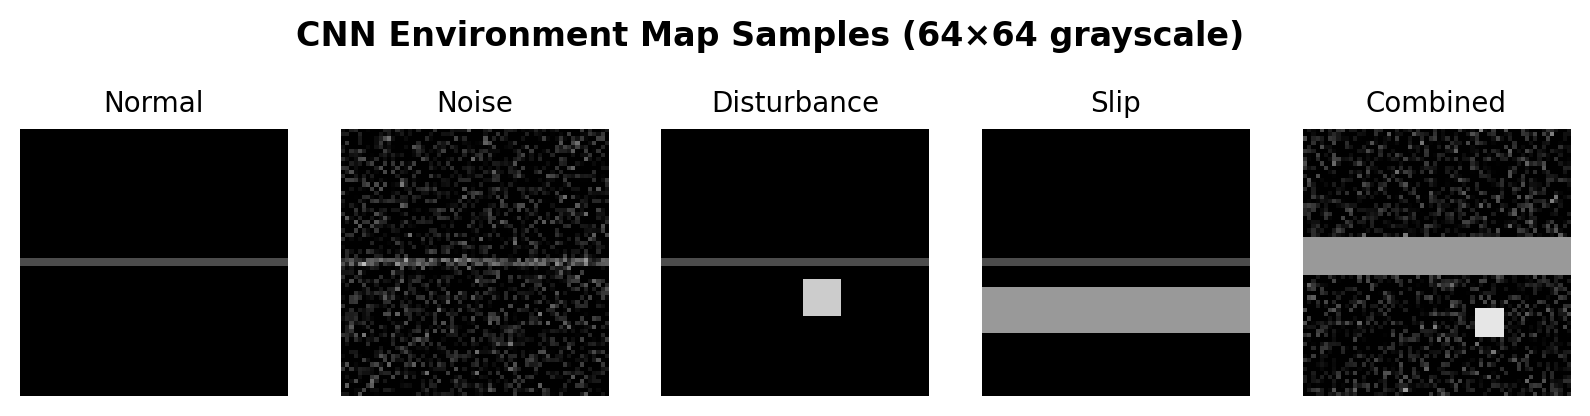
\includegraphics[width=0.95\textwidth]{../assets/figures/fig02_cnn_samples.png}
    \caption{Sample synthetic environment maps (one per class). Each $64{\times}64$
    grayscale image encodes a distinct visual signature used for CNN classification.}
    \label{fig:cnnsamples}
\end{figure}

\paragraph{Architecture (EnvironmentCNN).}
Three convolutional blocks, each comprising Conv2d ($3{\times}3$, padding 1) $\rightarrow$
BatchNorm $\rightarrow$ ReLU $\rightarrow$ MaxPool2d ($2{\times}2$), progressively produce
feature maps of depth 16, 32, and 64. The resulting $64{\times}8{\times}8$ representation
is flattened and processed by
$\text{FC}(4096 \to 128) \xrightarrow{\text{ReLU, Dropout}(0.3)} \text{FC}(128 \to 5)$.
Total trainable parameters: ${\approx}534$k. Training uses Adam (learning rate $10^{-3}$,
batch size 32) with cross-entropy loss over 20 epochs; the model reaches 100\% validation
accuracy by epoch 3.

\subsection{Adaptive Parameter Selection}

At deployment, the CNN classifies a pre-mission map and returns scenario label
$\hat{c} \in \{0, \dots, 4\}$. Each label maps to a hand-tuned parameter set
$\pi_{\hat{c}} = \{\lambda_x, \lambda_y, \lambda_\theta, k_v, k_\omega, \varphi,
\alpha_\omega\}$ (Table~\ref{tab:presets}). A first-order exponential filter prevents
abrupt gain jumps:
\begin{equation}
    \pi_k = (1 - \beta)\, \pi_{k-1} + \beta\, \pi_{\hat{c}}, \qquad \beta \in (0, 1] .
    \label{eq:filter}
\end{equation}

\begin{table}[ht]
    \centering
    \caption{Scenario-specific SMC parameter sets.}
    \label{tab:presets}
    \begin{tabular}{lccccc}
        \toprule
        \textbf{Param.} & \textbf{Normal} & \textbf{Noise} & \textbf{Dist.} & \textbf{Slip} & \textbf{Comb.} \\
        \midrule
        $\lambda_x$      & 2.00  & 2.00  & 2.15  & 2.20  & 2.15  \\
        $\lambda_y$      & 2.00  & 2.10  & 2.30  & 2.20  & 2.35  \\
        $\lambda_\theta$ & 1.00  & 0.95  & 1.05  & 1.00  & 1.00  \\
        $k_v$            & 0.30  & 0.30  & 0.33  & 0.35  & 0.35  \\
        $k_\omega$       & 0.80  & 0.78  & 0.88  & 0.86  & 0.88  \\
        $\varphi$        & 0.50  & 0.58  & 0.52  & 0.62  & 0.62  \\
        $\alpha_\omega$  & 0.950 & 0.965 & 0.945 & 0.960 & 0.965 \\
        \bottomrule
    \end{tabular}
\end{table}

The design rationale: \emph{Noise} widens the boundary layer ($\varphi = 0.58$) and raises
smoothing ($\alpha_\omega = 0.965$) to suppress chattering; \emph{Disturbance} increases
$\lambda_y$ and $k_\omega$ to restore heading quickly after an impulsive push; \emph{Slip}
elevates sliding-surface gains ($\lambda_x = \lambda_y = 2.20$) to compensate the velocity
deficit; \emph{Combined} balances smoothing and correction requirements.

\subsection{Reinforcement Learning Baseline (PPO)}

As an alternative to CNN supervision, a PPO agent (MLP policy, learning rate
$3 \times 10^{-4}$, $\gamma = 0.99$) observes a five-dimensional vector (instantaneous
tracking error, error rate, smoothed angular-velocity jitter, and noise/slip indicator
flags), selects one of the five parameter presets of Table~\ref{tab:presets} every 0.2\,s,
and receives reward $-e - 0.05\, j_\omega - 0.001\, |\omega_c|$ penalising tracking error
$e$ and chattering proxy $j_\omega$. Training uses 80k environment steps (40 episodes with
randomised scenarios) until the episode return plateaus.

\subsection{Stability Analysis}

Consider the composite Lyapunov candidate
\begin{equation}
    V = \tfrac{1}{2}\left( s_x^2 + s_y^2 + s_\theta^2 \right) \geq 0 .
    \label{eq:lyapunov}
\end{equation}
Differentiating along closed-loop trajectories and grouping bounded disturbances and
modelling residuals into $D(t)$ with $\|D(t)\| \leq \bd$ yields
\begin{equation}
    \dot{V} \leq -k_\omega \sum_{i \in \{y, \theta\}} s_i
        \tanh\!\left(\frac{s_i}{\varphi}\right) + \bd\, \|s\| .
    \label{eq:vdot}
\end{equation}
Because $|\tanh(\cdot)| \leq 1$ and $x\tanh(x/\varphi) \geq |x|\tanh(1) \approx 0.762|x|$
for $|x| \geq \varphi$, we have $\dot{V} < 0$ whenever $\|s\| > \bd / (0.762\, k_\omega)$,
establishing uniform ultimate boundedness (UUB) of the sliding surfaces. Inside the
boundary layer, the steady-state tracking error is bounded by
\begin{equation}
    \|e_i\|_\infty \leq \frac{\varphi + \bd/(\lambda_i k_\omega)}{\lambda_i} .
    \label{eq:uub}
\end{equation}
Equation~\eqref{eq:uub} reveals the design trade-off exploited by adaptive parameter
selection: a wider $\varphi$ reduces chattering at the cost of a larger ultimate error
bound, motivating the scenario-specific $\varphi$ values in Table~\ref{tab:presets}.

\subsection{Evaluation Protocol}

Both controllers track a straight-line reference at $v_r = 0.3$\,m/s for $T = 20$\,s
($\Delta t = 0.01$\,s, 2000 steps), starting aligned at the origin so deviations arise
solely from injected perturbations:
\begin{itemize}
    \item \textbf{Normal:} no perturbation.
    \item \textbf{Noise:} zero-mean Gaussian noise on $(x, y, \theta)$ measurements
          ($\sigma_{xy} = 0.02$\,m, $\sigma_\theta = 0.01$\,rad).
    \item \textbf{Disturbance:} single external push of $+0.4$\,m in $y$ at $t = 8$\,s.
    \item \textbf{Slip:} 30\% velocity reduction during $t \in [10, 14]$\,s.
    \item \textbf{Combined:} noise, disturbance, and slip simultaneously.
\end{itemize}
Metrics: RMSE tracking error, final tracking error at $t = T$, total control effort
($\sum |\omega_c|$), and chattering index (variance of successive $\omega_c$ differences).
All experiments are implemented in Python~3 (NumPy, PyTorch, Matplotlib) with fixed random
seeds and centralised YAML configuration. A web-based 3D digital twin (React + Three.js
frontend, FastAPI WebSocket backend) provides live visualisation, controller tours,
side-by-side dual comparison, simulation replay, and CSV export.

% ============================ RESULTS ============================
\section{Results}

\subsection{CNN Classification}

The EnvironmentCNN achieves 100\% test accuracy on 225 held-out simple-map samples
(precision/recall/F1 all 1.00). Perfect scores reflect engineered class separability, not
overfitting: validation loss falls jointly with training loss to near-zero by epoch 3 with
no divergence through epoch 20. Table~\ref{tab:classifiers} compares baseline classifiers
on the identical split, and reports the realistic-map evaluation: on procedurally
generated occupancy grids with border walls, random rectangular obstacles, and traversable
corridors, the retrained CNN reaches 95.1\% test accuracy --- comparable to published
robot perception classifiers \cite{ran2024,demirtas2024}.

\begin{table}[ht]
    \centering
    \caption{Classifier accuracy: simple vs.\ realistic maps (\%).}
    \label{tab:classifiers}
    \begin{tabular}{lcc}
        \toprule
        \textbf{Classifier} & \textbf{Simple} & \textbf{Realistic} \\
        \midrule
        $k$-NN ($k=5$)       & 48.44  & 41.33 \\
        Logistic regression  & 99.11  & 72.89 \\
        Random forest        & 100.00 & 98.22 \\
        EnvironmentCNN       & 100.00 & 95.11 \\
        \bottomrule
    \end{tabular}
\end{table}

\subsection{Trajectory and Tracking Performance}

Fig.~\ref{fig:trajectory} overlays robot trajectories under the combined scenario and
Fig.~\ref{fig:trackingerror} shows the corresponding tracking-error time series. The
adaptive controller recovers more tightly to the reference after the $t = 8$\,s push,
reducing final error from 20.9\,mm to 17.9\,mm ($-14.4\%$). Under sensor noise, the
angular-velocity command is markedly smoother for the adaptive controller, confirming the
chattering reduction predicted by the wider boundary layer.

\begin{figure}[ht]
    \centering
    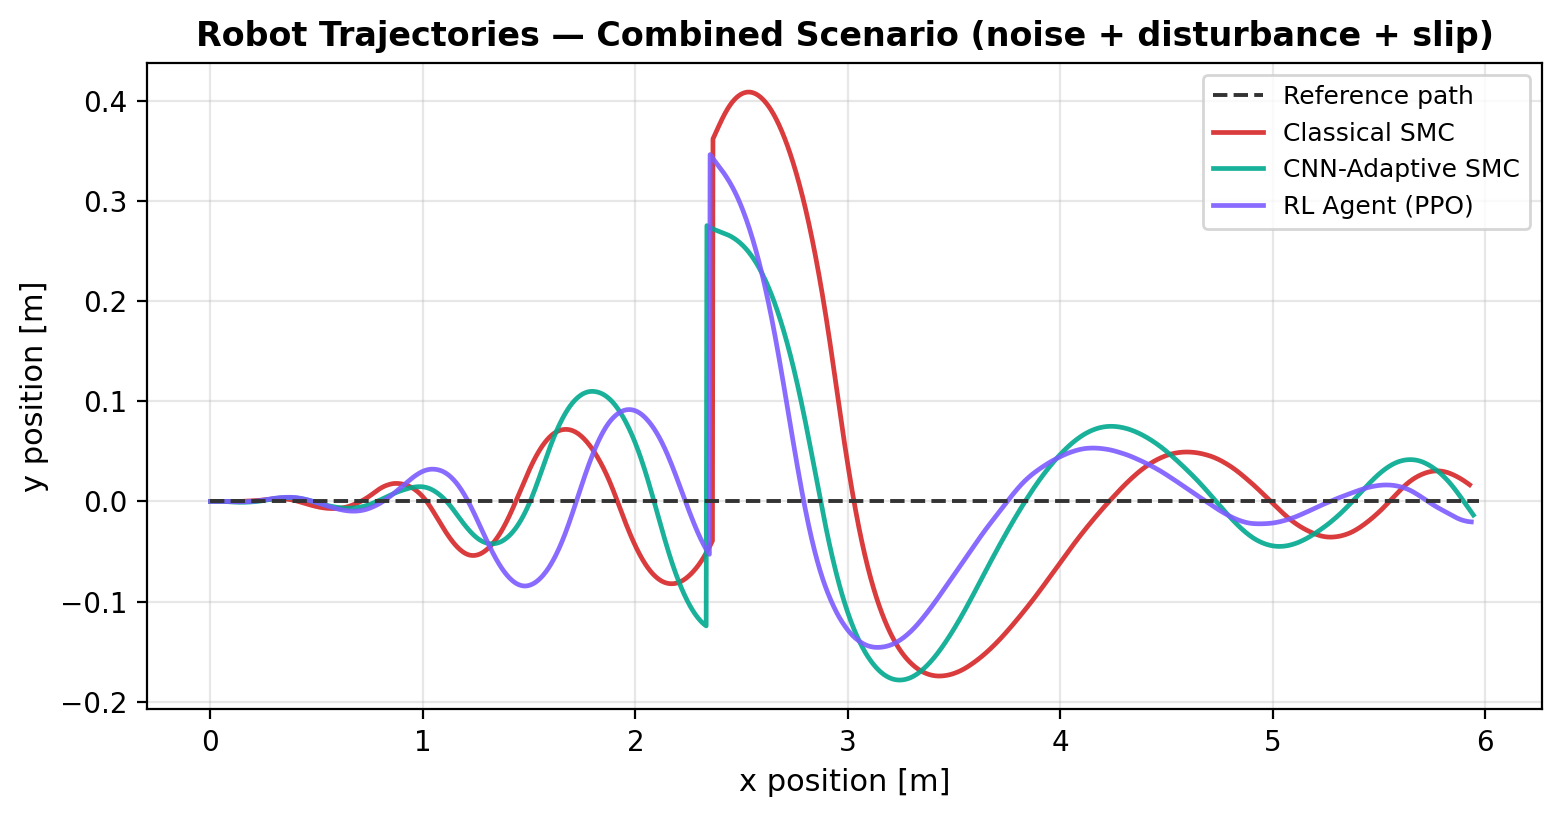
\includegraphics[width=0.92\textwidth]{../assets/figures/fig03_trajectory_comparison.png}
    \caption{Robot trajectories under combined uncertainty (noise + disturbance + slip)
    for all three controllers. The impulsive push at $t = 8$\,s ($x \approx 2.4$\,m) and
    the subsequent recovery are clearly visible; the adaptive controllers return to the
    reference more tightly than classical SMC.}
    \label{fig:trajectory}
\end{figure}

\begin{figure}[ht]
    \centering
    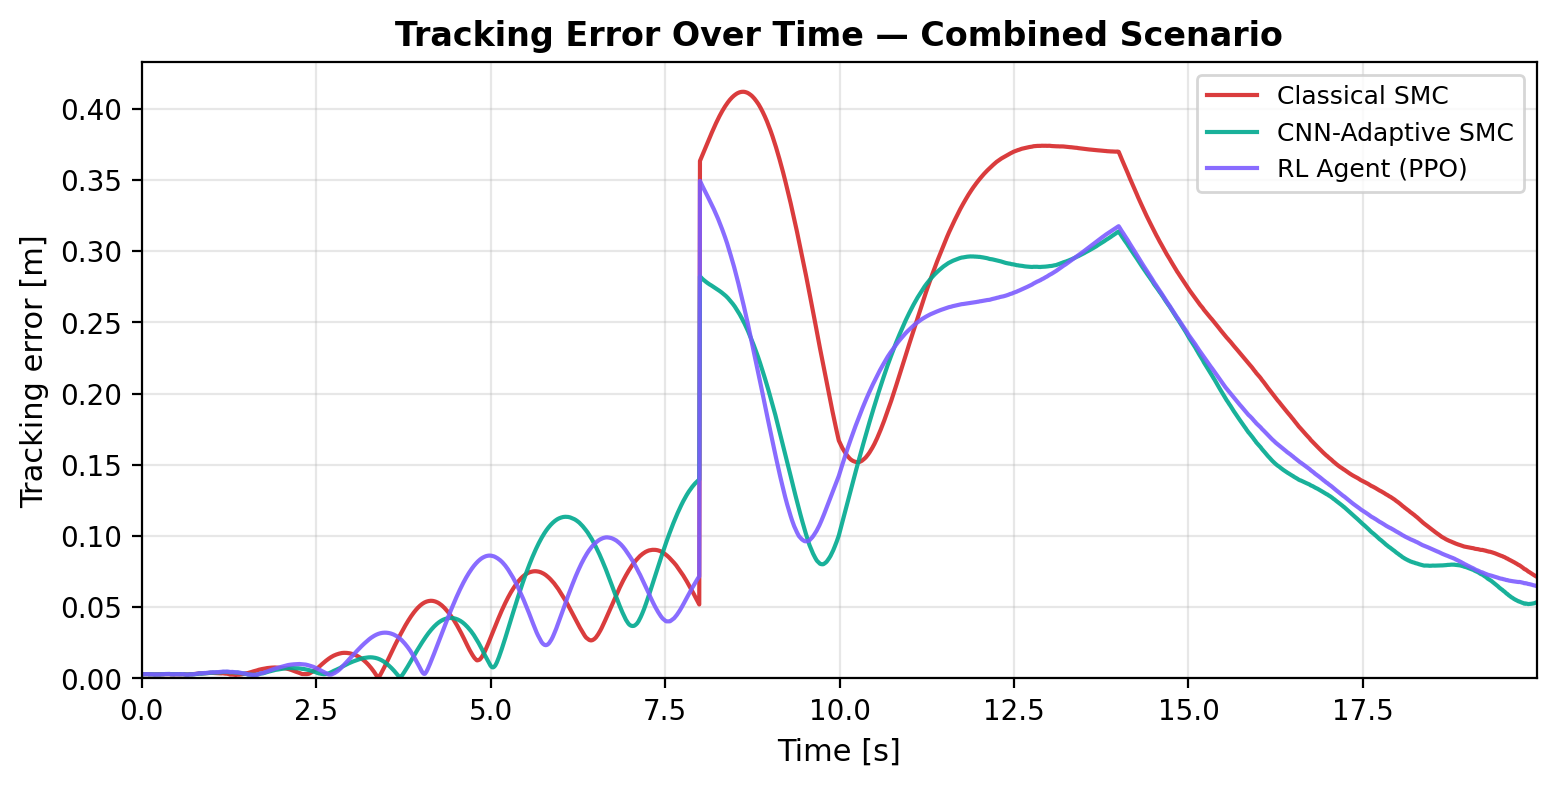
\includegraphics[width=0.92\textwidth]{../assets/figures/fig04_tracking_error.png}
    \caption{Tracking error over the full 20\,s episode under combined uncertainty. The
    disturbance impulse at $t = 8$\,s and the slip window $t \in [10, 14]$\,s are visible;
    the adaptive controllers decay faster after each perturbation.}
    \label{fig:trackingerror}
\end{figure}

\subsection{Quantitative Comparison}

Table~\ref{tab:absolute} reports absolute metric values for all scenarios;
Table~\ref{tab:improvement} summarises percentage improvements of the CNN-adaptive
controller over the classical baseline; and Table~\ref{tab:multicontroller} benchmarks
against fuzzy gain scheduling, oracle scenario selection, and RL-based preset selection
under identical conditions. Figs.~\ref{fig:rmsebars} and~\ref{fig:chatteringbars}
visualise the per-scenario comparison, Fig.~\ref{fig:heatmap} summarises the relative
improvements as a heatmap, and Fig.~\ref{fig:multicontroller} compares all five
controllers.

\begin{table}[ht]
    \centering
    \caption{Absolute controller metrics per scenario.}
    \label{tab:absolute}
    \begin{tabular}{llcccc}
        \toprule
        \textbf{Scenario} & \textbf{Ctrl.} & \textbf{RMSE (m)} & \textbf{Final (m)} & \textbf{Effort} & \textbf{Chatter} \\
        \midrule
        Normal      & Classical & 0.1465 & 0.0244 & 803.05 & 19.24 \\
                    & Adaptive  & 0.1465 & 0.0244 & 803.05 & 19.24 \\
        \addlinespace
        Noise       & Classical & 0.1599 & 0.0437 & 775.83 & 76.48 \\
                    & Adaptive  & 0.1786 & 0.1008 & 730.51 & 49.14 \\
        \addlinespace
        Disturbance & Classical & 0.1876 & 0.0209 & 874.45 & 15.74 \\
                    & Adaptive  & 0.1780 & 0.0179 & 923.15 & 17.83 \\
        \addlinespace
        Slip        & Classical & 0.1796 & 0.0407 & 577.12 & 7.88  \\
                    & Adaptive  & 0.1743 & 0.0274 & 640.25 & 9.72  \\
        \addlinespace
        Combined    & Classical & 0.2357 & 0.0650 & 673.99 & 70.87 \\
                    & Adaptive  & 0.2378 & 0.0642 & 705.86 & 51.65 \\
        \bottomrule
    \end{tabular}
\end{table}

\begin{table}[ht]
    \centering
    \caption{CNN-adaptive improvement over classical SMC (\%). $^{\dagger}$Under noise the
    final error increases in absolute terms (43.7\,mm $\to$ 100.8\,mm); this is the
    intentional smoothness--accuracy trade-off of Eq.~\eqref{eq:uub}, not a regression.}
    \label{tab:improvement}
    \begin{tabular}{lcccc}
        \toprule
        \textbf{Scenario} & \textbf{RMSE} & \textbf{Final Err.} & \textbf{Effort} & \textbf{Chattering} \\
        \midrule
        Normal      & 0.00     & 0.00                & 0.00     & 0.00     \\
        Noise       & $-11.65$ & $-130.62^{\dagger}$ & $+5.84$  & $+35.75$ \\
        Disturbance & $+5.12$  & $+14.42$            & $-5.57$  & $-13.32$ \\
        Slip        & $+2.94$  & $+32.69$            & $-10.94$ & $-23.40$ \\
        Combined    & $-0.85$  & $+1.20$             & $-4.73$  & $+27.12$ \\
        \bottomrule
    \end{tabular}
\end{table}

\begin{table}[ht]
    \centering
    \caption{Multi-controller comparison (selected metrics).}
    \label{tab:multicontroller}
    \begin{tabular}{llccccc}
        \toprule
        \textbf{Scenario} & \textbf{Metric} & \textbf{Class.} & \textbf{Fuzzy} & \textbf{CNN} & \textbf{Oracle} & \textbf{RL} \\
        \midrule
        Noise       & Chattering index & 76.48 & 70.50 & 49.14 & 49.32 & 50.72 \\
        Disturbance & Final err.\ (mm) & 20.92 & 24.75 & 17.90 & 15.58 & 32.75 \\
        Slip        & Final err.\ (mm) & 40.73 & 30.39 & 27.41 & 27.44 & 41.60 \\
        Combined    & Chattering index & 72.79 & 71.66 & 51.65 & 51.37 & 48.88 \\
        \bottomrule
    \end{tabular}
\end{table}

\begin{figure}[ht]
    \centering
    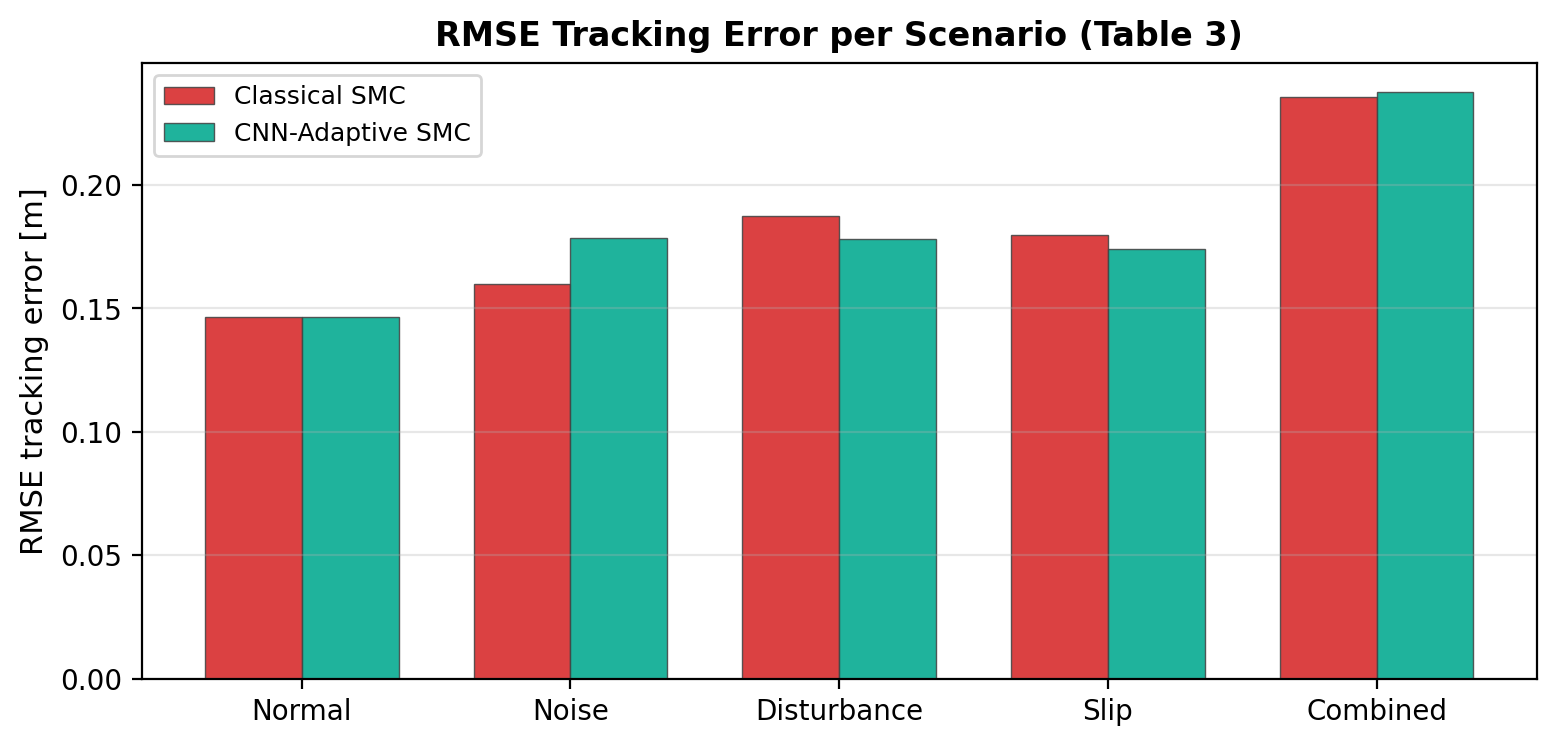
\includegraphics[width=0.92\textwidth]{../assets/figures/fig05_rmse_bars.png}
    \caption{RMSE tracking error across all five operating scenarios
    (values from Table~\ref{tab:absolute}).}
    \label{fig:rmsebars}
\end{figure}

\begin{figure}[ht]
    \centering
    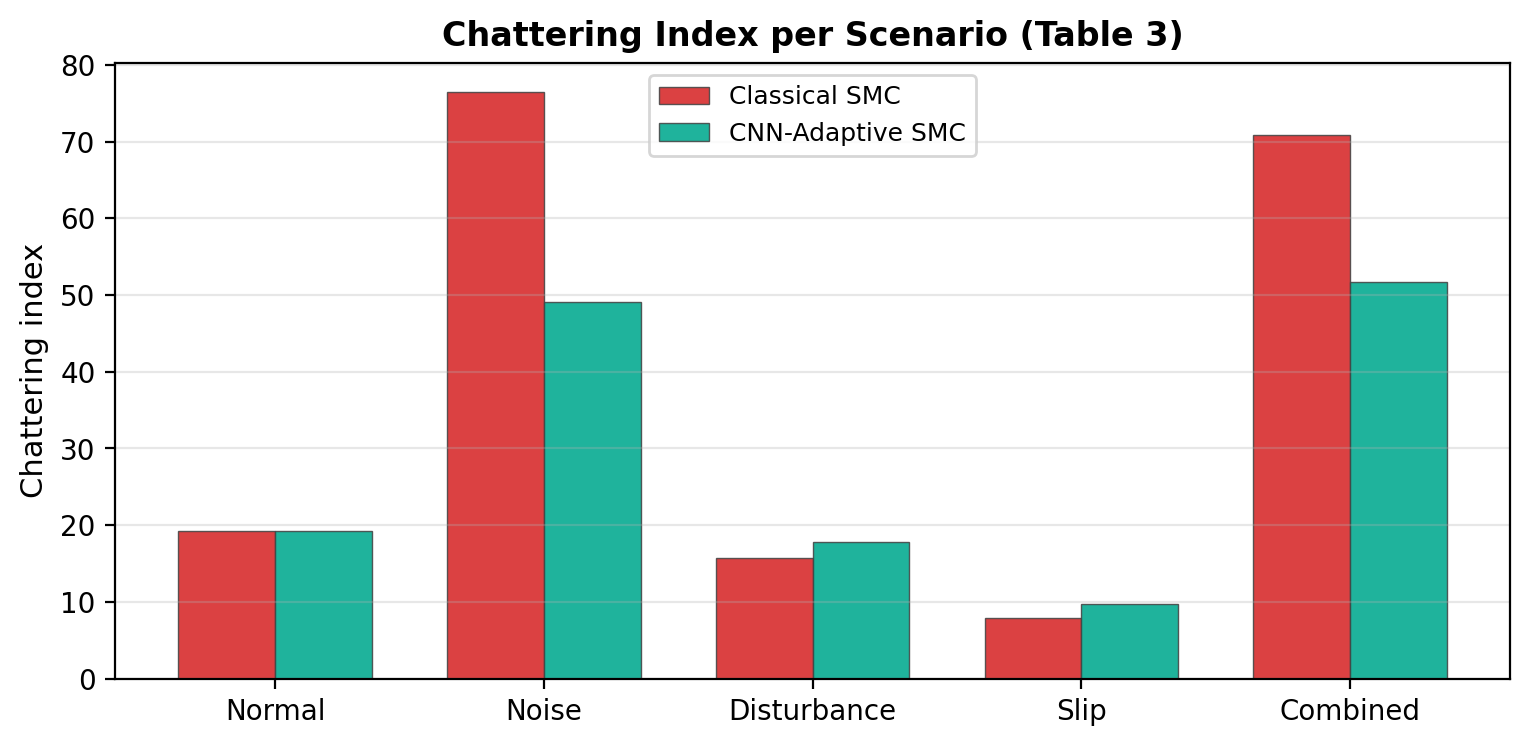
\includegraphics[width=0.92\textwidth]{../assets/figures/fig06_chattering_bars.png}
    \caption{Chattering index across scenarios (values from Table~\ref{tab:absolute}):
    CNN-adaptive SMC yields the largest reductions under noise and combined uncertainty.}
    \label{fig:chatteringbars}
\end{figure}

\begin{figure}[ht]
    \centering
    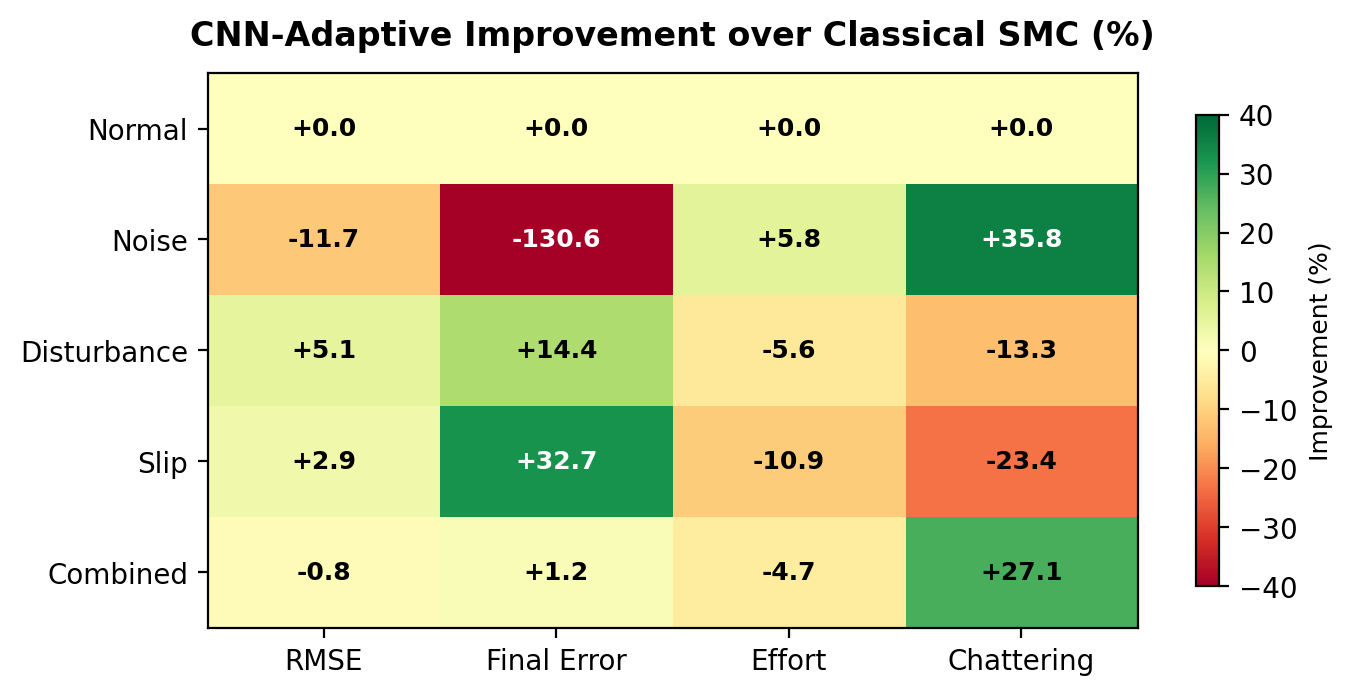
\includegraphics[width=0.85\textwidth]{../assets/figures/fig09_improvement_heatmap.png}
    \caption{Improvement heatmap of CNN-adaptive SMC over classical SMC (\%). Green =
    adaptive better; red = adaptive worse. The noise/final-error cell reflects the
    intentional smoothness--accuracy trade-off of Eq.~\eqref{eq:uub}.}
    \label{fig:heatmap}
\end{figure}

\begin{figure}[ht]
    \centering
    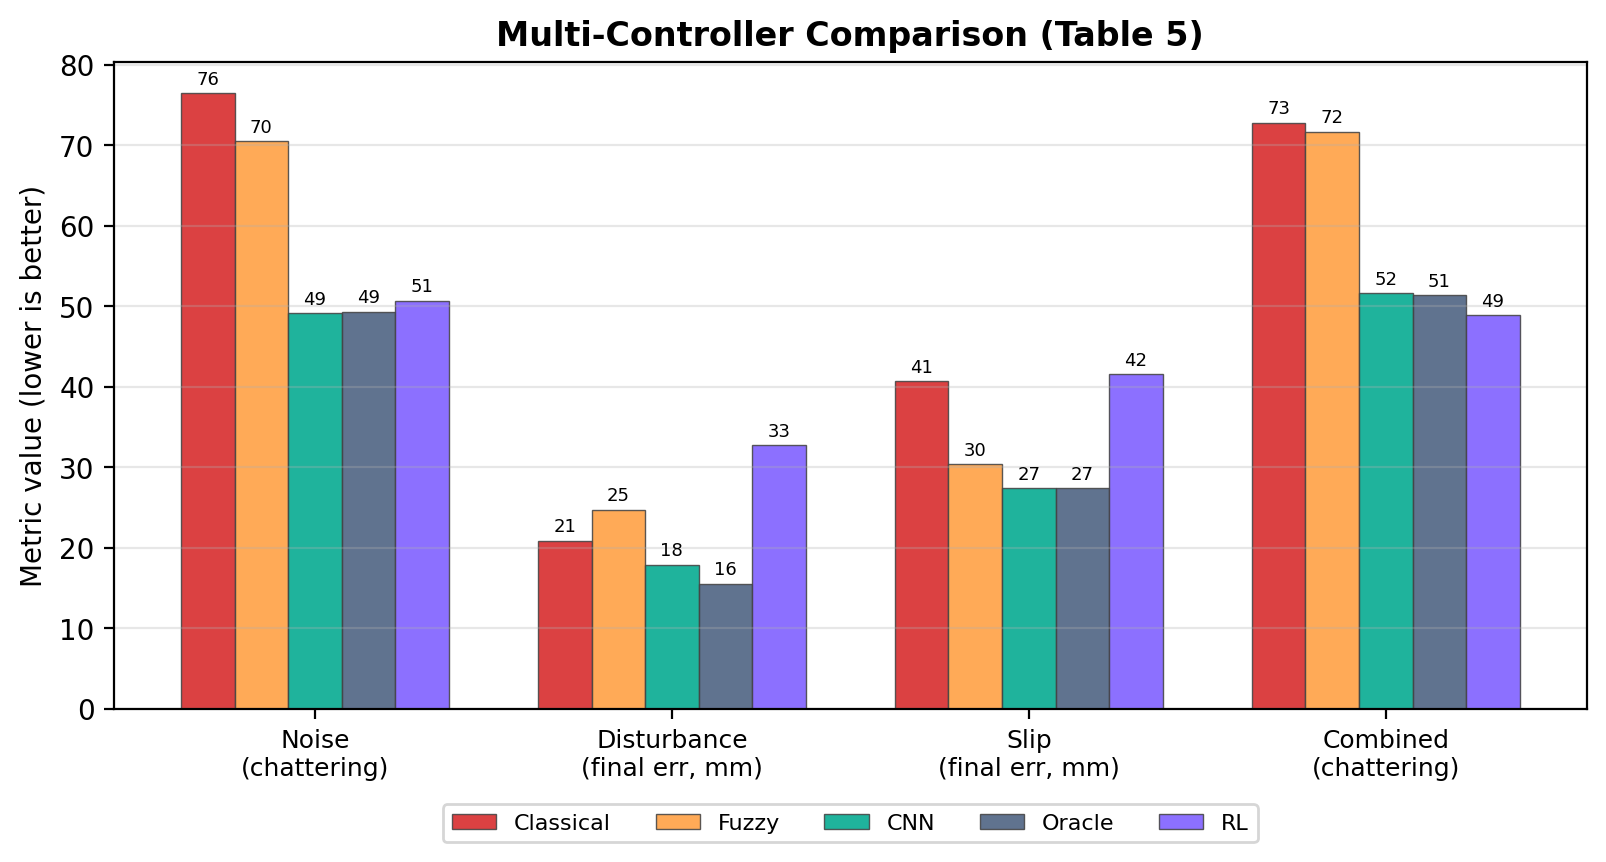
\includegraphics[width=0.95\textwidth]{../assets/figures/fig10_multicontroller.png}
    \caption{Multi-controller comparison across five controllers and four scenario/metric
    pairs (lower is better). CNN-adaptive and oracle presets achieve the largest
    reductions; RL is competitive under combined uncertainty.}
    \label{fig:multicontroller}
\end{figure}

\subsection{Discussion}

\paragraph{Alternative adaptive controllers.}
Fuzzy-SMC reduces chattering modestly under noise (70.5 vs.\ 76.5) but underperforms
CNN-adaptive and oracle selection on disturbance and slip recovery. Oracle selection
establishes the ceiling: 15.6\,mm final error under disturbance vs.\ 17.9\,mm for
CNN-adaptive, confirming that learned map classification is near-optimal on this
benchmark. RL-based selection achieves the lowest combined-scenario chattering (48.9) but
degrades under disturbance and slip, indicating that more training data and reward
shaping are needed before RL can replace the CNN supervisor.

\paragraph{Per-scenario analysis.}
\emph{Normal:} both controllers use identical parameters, so performance is equivalent by
construction --- a sanity check that the CNN classifies the unperturbed map correctly.
\emph{Noise:} chattering falls 35.7\% (76.48 $\to$ 49.14) via the wider boundary layer;
as predicted by Eq.~\eqref{eq:uub}, RMSE rises 11.7\% because smooth actuation is
prioritised over tight position holding. \emph{Disturbance:} stronger gains
($k_\omega = 0.88$, $\lambda_y = 2.30$) improve final error 14.4\%; the adaptive
controller settles within the 20\,mm threshold at $t = 18.3$\,s whereas the classical one
does not settle within the window. \emph{Slip:} elevated surface gains yield 32.7\%
final-error improvement at the cost of 10.9\% higher effort. \emph{Combined:} the hardest
case --- chattering falls 27.1\% with marginal final-error improvement, confirming that a
single static preset cannot simultaneously resolve all concurrent effects.

\paragraph{Computational considerations.}
The proposed scheme adds no runtime burden to the control loop: the CNN performs a single
pre-mission forward pass of a ${\approx}534$k-parameter network, after which the
controller executes the same closed-form update \eqref{eq:vc}--\eqref{eq:smoother} at
every 10\,ms step. The fuzzy baseline evaluates rule memberships every control step and
the RL baseline requires a policy forward pass every 0.2\,s, so the CNN-supervised
architecture is the cheapest adaptive variant at deployment time.

\subsection{Digital Twin Demonstration}

The 3D digital twin (Fig.~\ref{fig:twin}) provides live robot visualisation in a hospital
corridor environment, a controller tour (Classical $\to$ CNN $\to$ RL), side-by-side dual
comparison, simulation replay, and CSV export of metrics, with real-time WebSocket
streaming at adjustable simulation speed (1$\times$--5$\times$). It serves as the primary
demonstration vehicle for the project defense.

\begin{figure}[ht]
    \centering
    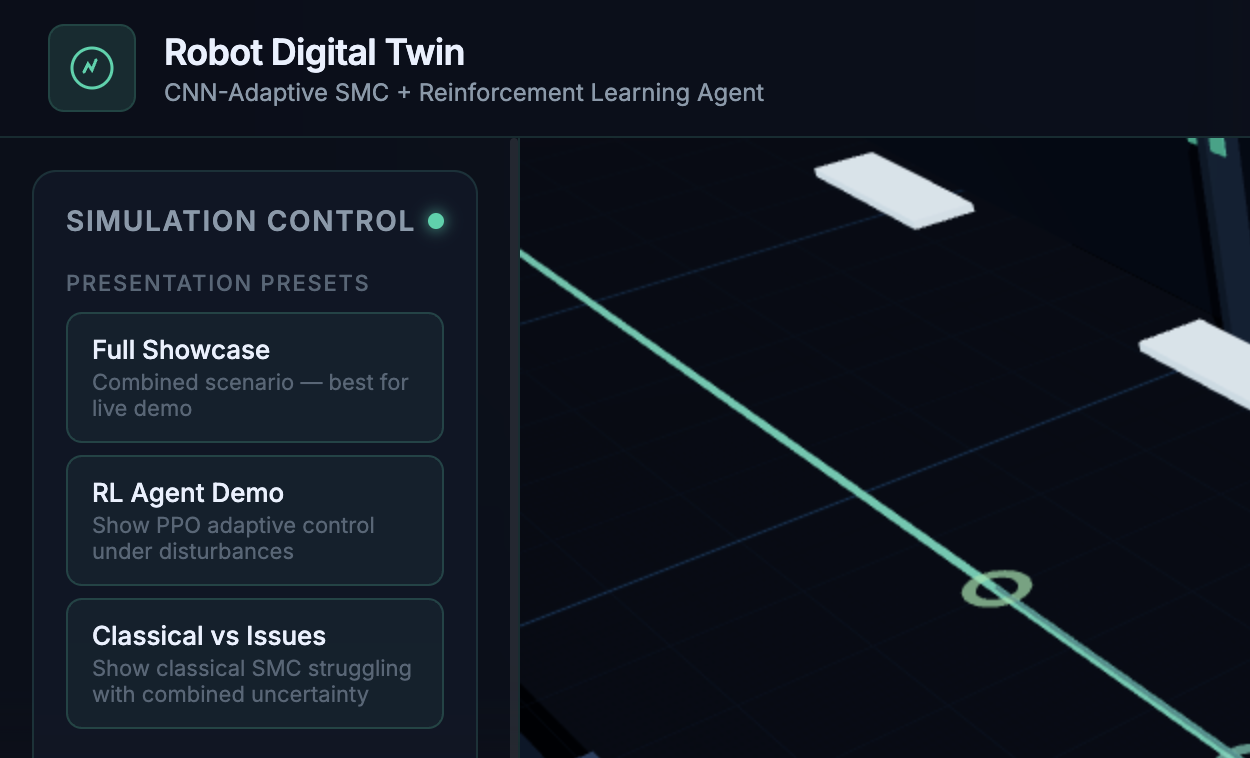
\includegraphics[width=0.92\textwidth]{../assets/figures/fig08_digital_twin.png}
    \caption{Screenshot of the live web-based 3D digital twin during a combined-scenario
    run (React + Three.js frontend, FastAPI WebSocket backend): control panel with
    presentation presets on the left, hospital-corridor 3D scene with the robot's
    trajectory trail on the right.}
    \label{fig:twin}
\end{figure}

% ============================ CONCLUSIONS ============================
\clearpage
\section{Conclusions}

This project presented a CNN-adaptive SMC framework for trajectory tracking of a simulated
differential-drive robot under five uncertainty conditions. A lightweight EnvironmentCNN
(${\approx}534$k parameters) classifies the operating environment from a $64{\times}64$
occupancy map and selects a corresponding SMC parameter set at run time, with exponential
smoothing to prevent gain discontinuities. A Lyapunov-based UUB analysis confirms that the
closed-loop system is uniformly ultimately bounded under bounded disturbances, and that
the steady-state error bound is directly parameterised by the boundary-layer width
$\varphi$, providing theoretical grounding for the scenario-specific presets.

Simulation results across five scenarios confirm:
\begin{itemize}
    \item \textbf{35.7\%} chattering reduction under sensor noise (76.48 $\to$ 49.14),
          with expected steady-state error widening per Eq.~\eqref{eq:uub};
    \item \textbf{14.4\%} improvement in final tracking-error recovery after external
          disturbance (20.9\,mm $\to$ 17.9\,mm), within 2.3\,mm of the oracle upper bound;
    \item \textbf{32.7\%} improvement in final error under wheel slip
          (40.7\,mm $\to$ 27.4\,mm);
    \item near-oracle performance across fuzzy, RL, and classical baselines, with
          \textbf{95.1\%} CNN accuracy on realistic maps;
    \item a fully operational 3D digital twin integrating all controllers with live
          benchmarking, replay, and export.
\end{itemize}

\paragraph{Limitations.}
The CNN operates on synthetic maps with engineered class separability and performs a
single pre-mission classification rather than continuous on-line inference. Adaptive
parameters are hand-tuned per scenario rather than learned end-to-end. The evaluation is
restricted to a straight-line trajectory in a 2-D kinematic simulation with single fixed
random seeds rather than Monte-Carlo repetitions.

\paragraph{Future Work.}
(i) Replace synthetic maps with real LiDAR-based occupancy grids (the realistic-map CNN
already reaches 95.1\%); (ii) deploy continuous on-line scenario inference so the
controller reacts to mid-mission condition changes; (iii) extend RL training with larger
scenario randomisation and multi-objective rewards; (iv) evaluate on curved and waypoint
trajectories with Monte-Carlo repetitions to attach confidence intervals; (v) validate on
a physical differential-drive robot.

\section*{Code Availability}
The complete simulation framework, CNN training pipeline, dataset generation scripts, and
digital twin are available at
\url{https://github.com/LikhitaYerra/smc_cnn}.

% ============================ REFERENCES ============================
\begin{thebibliography}{12}

\bibitem{utkin1992}
V.~I. Utkin, \emph{Sliding Modes in Control and Optimization}. Springer-Verlag, Berlin, 1992.

\bibitem{edwards1998}
C.~Edwards and S.~K. Spurgeon, \emph{Sliding Mode Control: Theory and Applications}.
Taylor \& Francis, London, 1998.

\bibitem{shtessel2014}
Y.~Shtessel, C.~Edwards, L.~Fridman, and A.~Levant, \emph{Sliding Mode Control and
Observation}. Birkh\"auser, New York, 2014.

\bibitem{slotine1991}
J.-J.~E. Slotine and W.~Li, \emph{Applied Nonlinear Control}. Prentice Hall,
Englewood Cliffs, NJ, 1991.

\bibitem{lin2006}
F.-J. Lin and P.-H. Shen, ``Robust fuzzy neural network sliding-mode control for two-axis
motion control system,'' \emph{IEEE Trans. Ind. Electron.}, vol.~53, no.~4,
pp. 1209--1225, Jun. 2006.

\bibitem{ge2004}
S.~S. Ge and C.~Wang, ``Adaptive neural control of uncertain MIMO nonlinear systems,''
\emph{IEEE Trans. Neural Netw.}, vol.~15, no.~3, pp. 674--692, May 2004.

\bibitem{lecun2015}
Y.~LeCun, Y.~Bengio, and G.~Hinton, ``Deep learning,'' \emph{Nature}, vol.~521,
pp. 436--444, May 2015.

\bibitem{levine2016}
S.~Levine, C.~Finn, T.~Darrell, and P.~Abbeel, ``End-to-end training of deep visuomotor
policies,'' \emph{J. Mach. Learn. Res.}, vol.~17, no.~39, pp. 1--40, 2016.

\bibitem{nguyen2018}
N.~P. Nguyen and S.~K. Hong, ``Sliding mode Thau observer for actuator fault diagnosis of
quadcopter UAVs,'' \emph{Appl. Sci.}, vol.~8, no.~10, p.~1893, 2018.

\bibitem{liberzon2003}
D.~Liberzon, \emph{Switching in Systems and Control}. Birkh\"auser, Boston, MA, 2003.

\bibitem{ran2024}
Y.~Ran, X.~Xu, M.~Luo, J.~Yang, and Z.~Chen, ``Scene classification method based on
multi-scale convolutional neural network with long short-term memory and whale
optimization algorithm,'' \emph{Remote Sens.}, vol.~16, no.~1, p.~174, Jan. 2024.

\bibitem{demirtas2024}
A.~Demirta\c{s}, G.~Erdemir, and H.~Bayram, ``Indoor surface classification for mobile
robots,'' \emph{PeerJ Comput. Sci.}, vol.~10, p.~e1730, Jan. 2024.

\end{thebibliography}

\end{document}
